\chapter{Referencial teórico}
\label{cap:referencial_teorico}

Faça uma compilação dos principais autores sobre o tema a ser investigado. Nesta fase é importante o apoio de seu orientador e a clareza quanto ao tema e à pergunta da sua pesquisa, indicando o que é essencial ser lido e resumido e o que é secundário. A pergunta funciona como um guia do que deve ser exposto nesse capítulo e, principalmente, do que não é necessário.

A forma pela qual você estruturará esse capítulo já será uma de suas contribuições. Cada pesquisador, dentro de um mesmo tema, possui uma forma única de organizar o conhecimento compulsado. 

O Referencial teórico é como uma aula sobre o tema para que o leitor consiga acompanhar os próximos capítulos de seu trabalho. Observe que não é um resumo de tudo que você aprendeu no seu curso.

Divida o assunto que você deseja estudar em seções. As seções devem conduzir o leitor pelos conceitos apresentados. Assim, você deve começar pelo tópico mais geral e ir especificando cada vez mais até trazer seu leitor ao tema específico de seu trabalho acadêmico. Dentro de cada seção, você pode usar subseções para organizar melhor a informação destacada.

\section{Assunto mais geral do referencial teórico} \label{sub:assunto2}

A primeira seção do referencial teórico normalmente será sobre o tema mais geral dentre os assuntos abordados no seu trabalho. 

\section{Assunto mais específico do referencial teórico}

As demais sessões tendem a ser mais específicas que as anteriores

\section{Trabalhos relacionados}

Nessa seção, você pode elencar os trabalhos com os quais as suas contribuições podem ser comparadas na seção de discussão ao final do seu documento.
Para que o leitor entenda as similaridades entre seu trabalho e os trabalhos correlatos, você deve, aqui, fazer um resumo de cada trabalho correlato realçando a interseção que eles possuem com os seus objetivos de pesquisa.

\section{Quadro referencial teórico}

Você pode incluir um quadro ao final do seu referencial destacando para o leitor quais foram as suposições ou hipóteses construídas a partir da literatura que você compilou. A palavra hipótese é mais utilizada em pesquisas quantitativas. A palavra suposição é mais utilizada em pesquisas mais interpretativas, qualitativas.

O trabalho \cite{DissertacaoElton2015}, por utilizar uma metodologia mista, apresenta exemplos de quadro de hipóteses e de quadro de suposições. A figura~\ref{fig:quadro_hipoteses} apresenta uma parte do quadro de hipóteses do trabalho. 

\begin{figure}[ht]
    \centering
    \caption{Parte de um quadro de hipóteses.}
    \copyrightbox[b]
    		{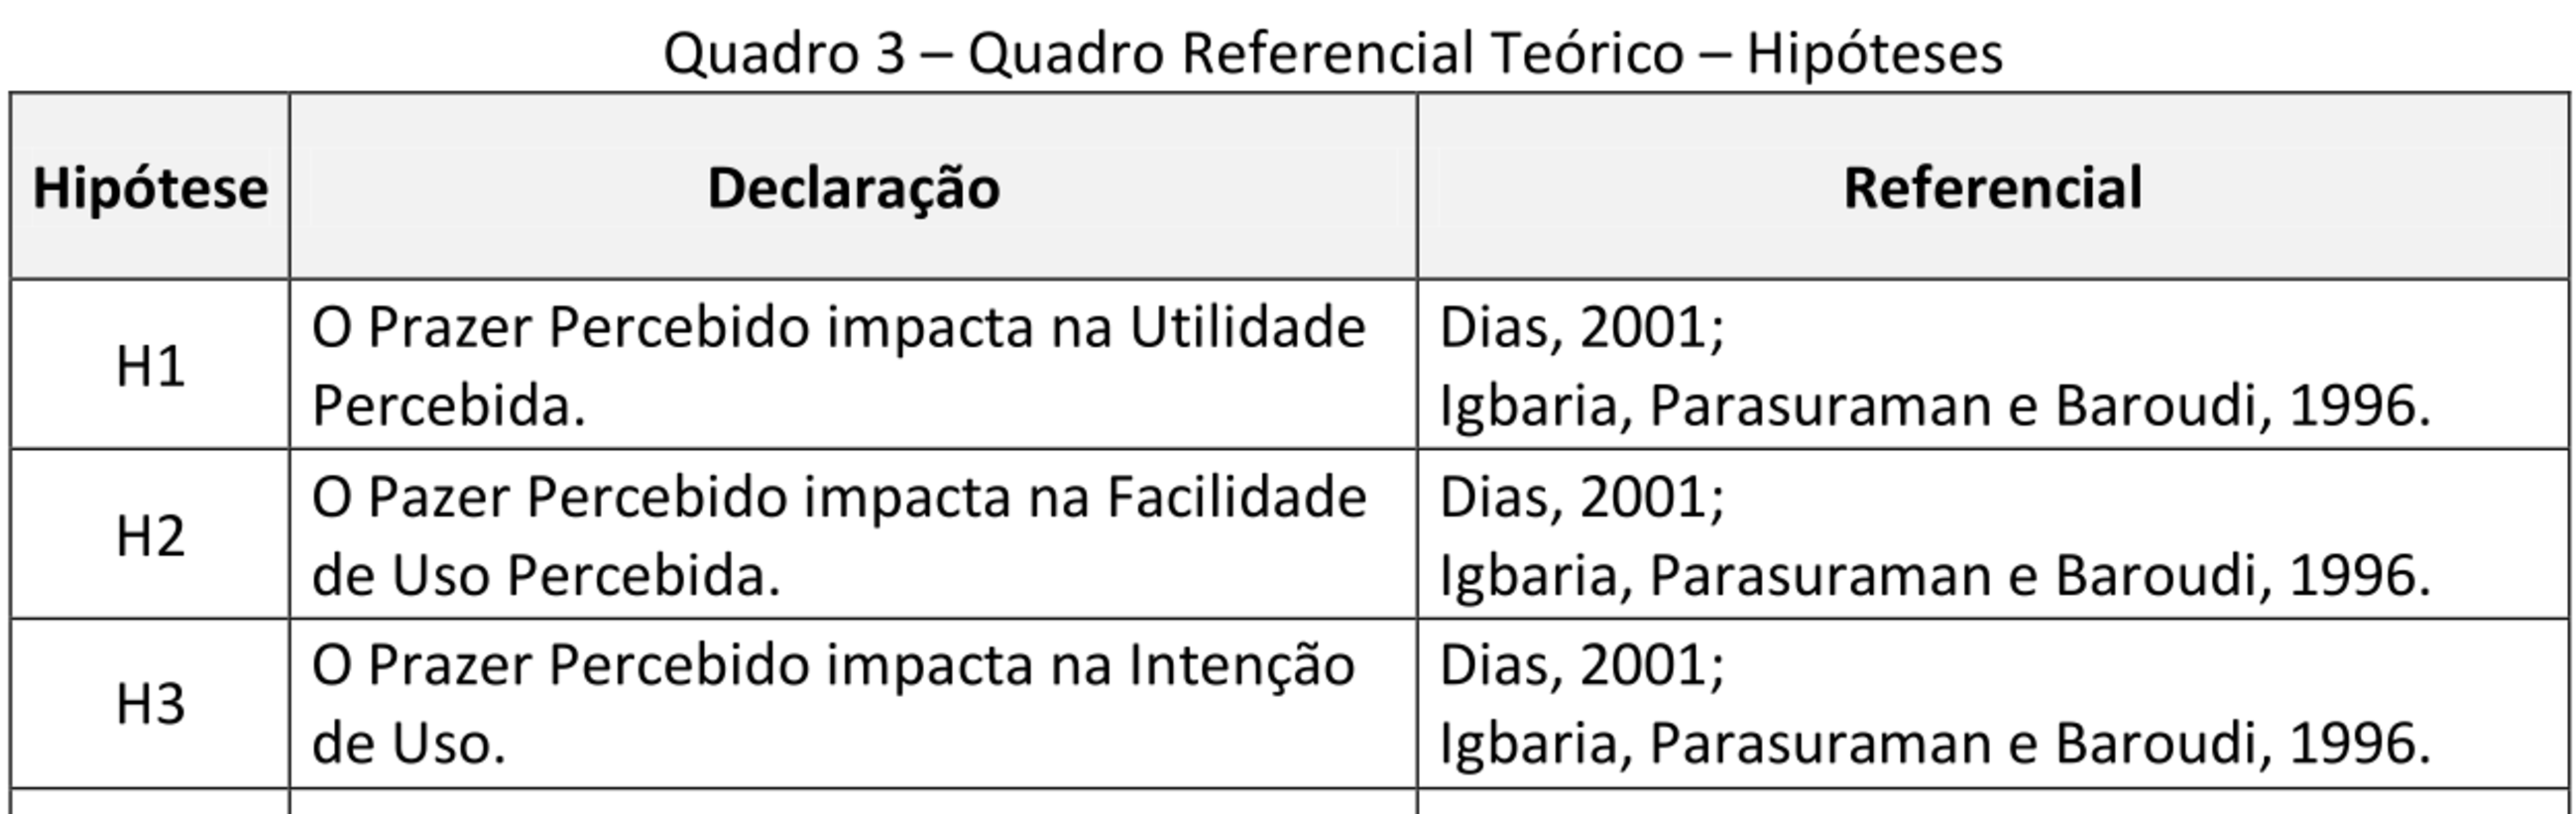
\includegraphics[width=1\linewidth]{quadro_hipotese}}
            {Fonte: Extraída de \cite[37]{DissertacaoElton2015}}
    \label{fig:quadro_hipoteses}
\end{figure}

Ainda sobre o mesmo trabalho, a figura~\ref{fig:quadro_suposicoes} apresenta uma parte do quadro de suposições.

\begin{figure}[ht]
    \centering
    \caption{Parte de um quadro de suposições}
    \copyrightbox[b]
  		{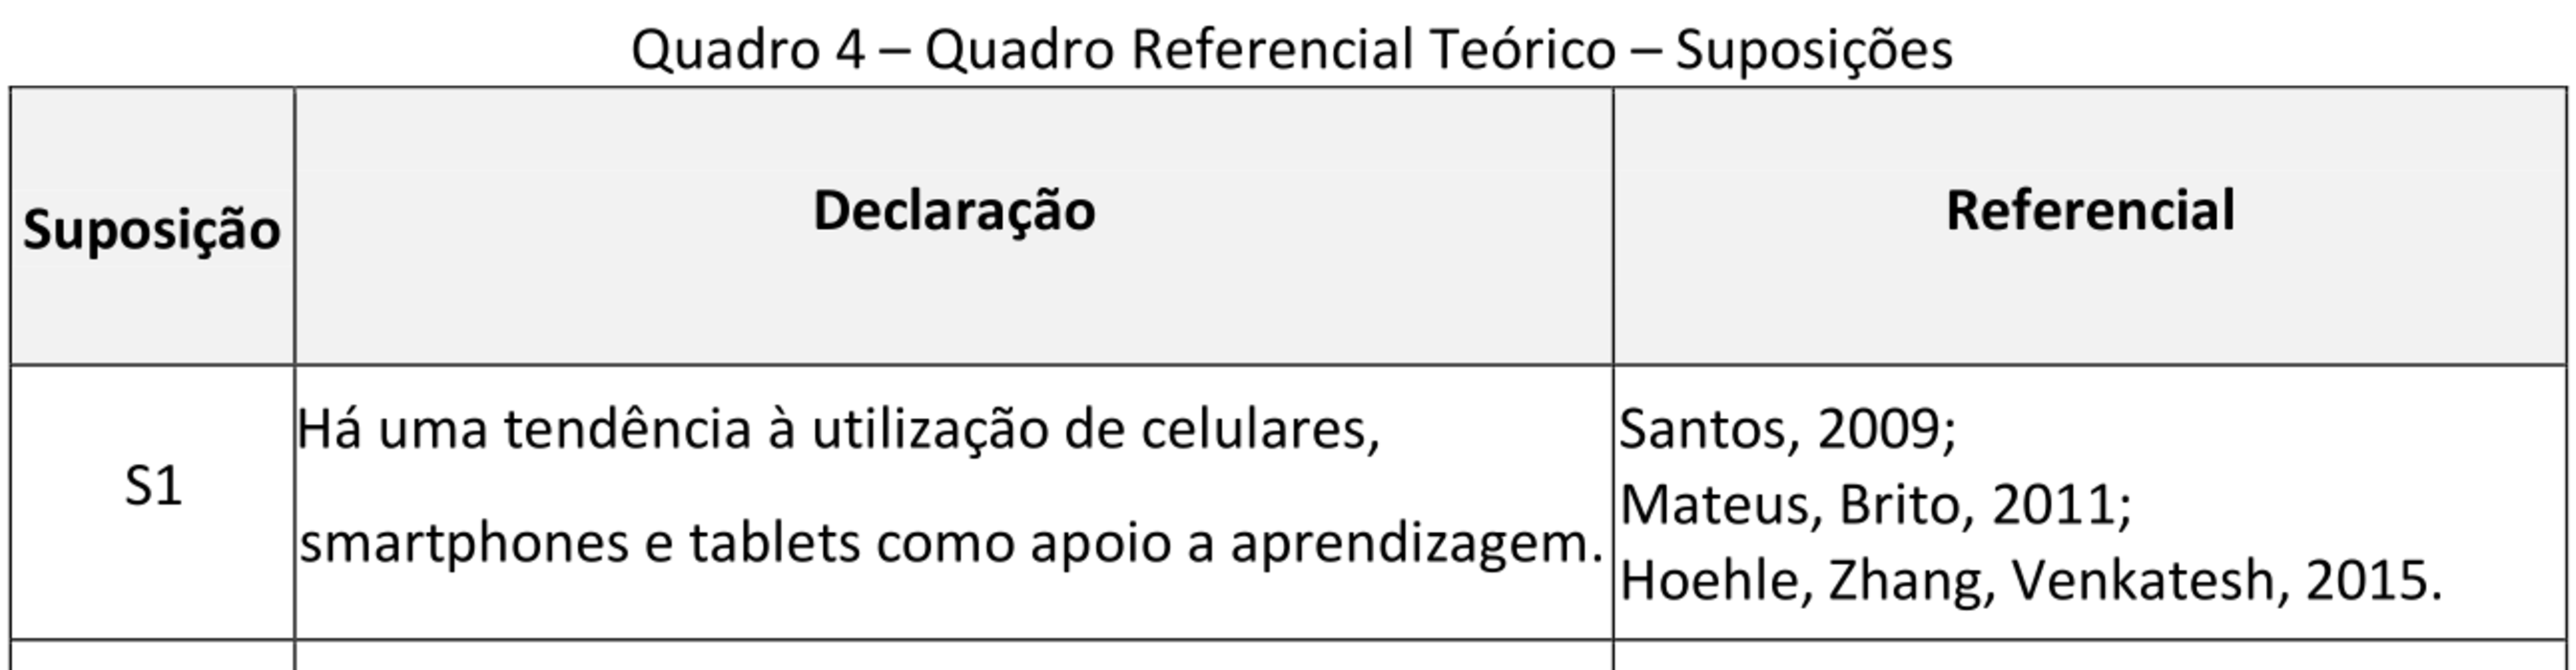
\includegraphics[width=1\linewidth]{quadro_suposicao}}
        {Fonte: Extraída de \cite[38]{DissertacaoElton2015}}
    \label{fig:quadro_suposicoes}
\end{figure}